\documentclass{beamer}
\usepackage[utf8]{inputenc}

\usetheme{Madrid}
\usecolortheme{default}
\usepackage{amsmath,amssymb,amsfonts,amsthm}
\usepackage{mathtools}
\usepackage{txfonts}
\usepackage{tkz-euclide}
\usepackage{listings}
\usepackage{adjustbox}
\usepackage{array}
\usepackage{gensymb}
\usepackage{tabularx}
\usepackage{gvv}
\usepackage{lmodern}
\usepackage{circuitikz}
\usepackage{tikz}
\lstset{literate={·}{{$\cdot$}}1 {λ}{{$\lambda$}}1 {→}{{$\to$}}1}
\usepackage{multicol}
\usepackage{graphicx}

\setbeamertemplate{page number in head/foot}[totalframenumber]

\usepackage{tcolorbox}
\tcbuselibrary{minted,breakable,xparse,skins}



\definecolor{bg}{gray}{0.95}
\DeclareTCBListing{mintedbox}{O{}m!O{}}{%
  breakable=true,
  listing engine=minted,
  listing only,
  minted language=#2,
  minted style=default,
  minted options={%
    linenos,
    gobble=0,
    breaklines=true,
    breakafter=,,
    fontsize=\small,
    numbersep=8pt,
    #1},
  boxsep=0pt,
  left skip=0pt,
  right skip=0pt,
  left=25pt,
  right=0pt,
  top=3pt,
  bottom=3pt,
  arc=5pt,
  leftrule=0pt,
  rightrule=0pt,
  bottomrule=2pt,
  toprule=2pt,
  colback=bg,
  colframe=orange!70,
  enhanced,
  overlay={%
    \begin{tcbclipinterior}
    \fill[orange!20!white] (frame.south west) rectangle ([xshift=20pt]frame.north west);
    \end{tcbclipinterior}},
  #3,
}
\lstset{
    language=C,
    basicstyle=\ttfamily\small,
    keywordstyle=\color{blue},
    stringstyle=\color{orange},
    commentstyle=\color{green!60!black},
    numbers=left,
    numberstyle=\tiny\color{gray},
    breaklines=true,
    showstringspaces=false,
}
%------------------------------------------------------------
%This block of code defines the information to appear in the
%Title page
\title %optional
{12.768}
\date{October 10,2025}
%\subtitle{A short story}

\author % (optional)
{Harsha-EE25BTECH11026}



\begin{document}


\frame{\titlepage}


\begin{frame}{Question}
In the figure, the vectors $\vec{u}$ and $\vec{v}$ are related as $\vec{A}\vec{u}=\vec{v}$ by a transformation matrix $\vec{A}$. The correct choice of $\vec{A}$ is
\begin{enumerate}
\begin{multicols}{4}
    \item $\myvec{\tfrac{4}{5}&&\tfrac{3}{5}\\\tfrac{3}{5}&&-\tfrac{4}{5}}$
    \item $\myvec{\tfrac{4}{5}&&-\tfrac{3}{5}\\\tfrac{3}{5}&&\tfrac{4}{5}}$
    \item $\myvec{\tfrac{4}{5}&&\tfrac{3}{5}\\-\tfrac{3}{5}&&\tfrac{4}{5}}$
    \item $\myvec{\tfrac{4}{5}&&-\tfrac{3}{5}\\\tfrac{3}{5}&&-\tfrac{4}{5}}$
\end{multicols}
\end{enumerate}
\end{frame}
\begin{frame}{Question}
    \begin{figure}[H]
    \centering
    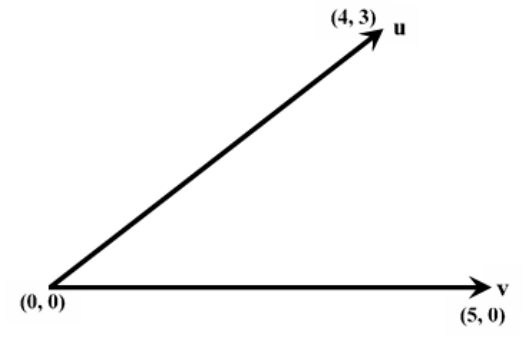
\includegraphics[width=0.4\columnwidth]{figs/Fig-1.png}
    \caption{Figure-1}
    \label{fig:1}
\end{figure}
\end{frame}


\begin{frame}{Theoretical solution}
    Given,
\begin{align}
    \vec{u}=\myvec{4\\3} \qquad \vec{v}=\myvec{5\\0}
\end{align}
From ~\ref{fig:1},
\begin{align}
    \|\vec{u}\|=\|\vec{v}\|=5 \; units
\end{align}
This implies, $\vec{A}$ is a rotation matrix.\\
Rotation matrix $\vec{A}$ is given by 
\begin{align}
    \vec{A}=\myvec{\cos{\theta}&&-\sin{\theta}\\\sin{\theta}&&\cos{\theta}}
\end{align}
where $\theta$ is the angle between the vectors in counter-clockwise sense.
\end{frame}

\begin{frame}{Theoretical solution}
    \begin{align}
    \therefore \myvec{\cos{\theta}&&-\sin{\theta}\\\sin{\theta}&&\cos{\theta}}\myvec{4\\3}=\myvec{5\\0}
\end{align}
\begin{align}
    \myvec{4\cos{\theta}-3\sin{\theta}\\4\sin{\theta}+3\cos{\theta}}=\myvec{5\\0}
\end{align}
The above equation can be re-arranged as,
\begin{align}
    \myvec{4&&-3\\3&&4}\myvec{\cos{\theta}\\\sin{\theta}}=\myvec{5\\0}
    \label{eq:1}
\end{align}
We need to solve for $\cos{\theta}$ and $\sin{\theta}$ to get the transformation matrix $\vec{A}$.
\end{frame}

\begin{frame}{Theoretical solution}
We can see that in ~\eqref{eq:1}, the columns of the coefficient matrix are orthogonal to each other and also the column vectors have the same norm.
\begin{align}
    \therefore \frac{1}{5}\myvec{4&&-3\\3&&4}\myvec{\cos{\theta}\\\sin{\theta}}=\frac{1}{5}\myvec{5\\0}
\end{align}
\begin{align}
    \implies \myvec{\tfrac{4}{5}&&-\tfrac{3}{5}\\\tfrac{3}{5}&&\tfrac{4}{5}}\myvec{\cos{\theta}\\\sin{\theta}}=\myvec{1\\0}
    \label{eq:2}
\end{align}
In equation ~\eqref{eq:2}, the coefficient matrix is an orthogonal matrix.
\begin{align}
    \implies \vec{A}\vec{x}=\vec{b} 
    \Rightarrow 
    \vec{A}^{\top}\vec{A}\vec{x}=\vec{A}^{\top}\vec{b}
    \Rightarrow
    \vec{x}=\vec{A}^{\top}\vec{b} \qquad \brak{\because \vec{A}^{\top}\vec{A}=\vec{I}}
\end{align}
\end{frame}

\begin{frame}{Theoretical solution}
\begin{align}
    \therefore \myvec{\cos{\theta}\\\sin{\theta}}=\myvec{\tfrac{4}{5}&&\tfrac{3}{5}\\-\tfrac{3}{5}&&\tfrac{4}{5}}\myvec{1\\0}
\end{align}
\begin{align}
    \therefore \myvec{\cos{\theta}\\\sin{\theta}}=\myvec{\tfrac{4}{5}\\-\tfrac{3}{5}}
\end{align}
\begin{align}
    \implies \vec{A}=\myvec{\tfrac{4}{5}&&\tfrac{3}{5}\\-\tfrac{3}{5}&&\tfrac{4}{5}}
\end{align}
\end{frame}





\end{document}